\chapter{Introduction}

\label{sec:intro}

The early investigations  of elementary particles at the beginning of the 20th century, have brought up a radically new theoretical approach, which describes the observed phenomena by gauge symmetry groups. This concept is better known as the Standard Model of elementary particle physics (SM) (see~\cref{sec:SM1}).

The SM has undergone extensive investigations of its properties, which confirm its consistency astonishingly well. Despite the remarkable success of the SM, there are still a lot of open questions. For example astronomical observations  bring up concepts, which are hints that the SM in its present form might not be complete. The constraining of the SM  is a very important task and the investigation of the top-quark might bring up some interesting results in this context. 

The discovery of the top-quark completes the so called quark sector of the SM, which groups one specific particle type. In comparison with the other quarks however, the properties of the top quark are outstanding. A very good example  is its mass $m_{\text{top}}$, which is about forty times larger than the mass of the second heaviest quark, the bottom quark. Furthermore, $m_{\text{top}}$ is a fundamental parameter of the SM, which has huge impact on certain quantities, like the stability of SM vacuum.  Thus, it is very interesting to investigate this property.

As displayed by~\cref{fig:mass} there have been several measurements of the top-quark mass performed by the CMS and ATLAS collaboration~\cite{PubR}. The shown results belong to different decay channels. Furthermore, the current world average value of 173.55 $\pm$ 0.5~GeV is displayed (orange)~\cite{ATLAS:2014wva}, which also takes the results from the Tevatron measurements into account. Several measurements (green) have been performed by the ATLAS group of the Max-Planck-Institute for Physics in Munich (MPP). All these results stem from the so-called dileptonic decay and the lepton+jets decay channel. At the MPP, the measurements of the top-quark mass in both of this channels were performed for a center-of-mass energy of 7 and 8~TeV~\cite{Aad:2015nba,Aaboud:2016igd,ATLAS-CONF-2017-071}. The latest combination value of these two decay channels, for the  8~TeV results (grey), yields to a top-quark mass value of 172.51 $\pm$ 0.5~GeV~\cite{ATLAS-CONF-2017-071}.

For this analysis, the $t\bar{t}\rightarrow$lepton + jets channel is used. 
In events of this kind, a top-antitop quark pair is produced. One of the these quarks decays into a lepton pair, and a $b$ quark, while the second one decays into a $b$ quark  and additional light quarks. The $b$ quarks and the light quarks trigger  particle showers, which can be identified with the experiment as hadronic jets. 
The basic idea of this thesis is to perform the  
$m_{	\rm top}$ measurement, in the same way as it was done in the previous analyses~\cite{Aad:2015nba,ATLAS-CONF-2017-071}, using the so-called template method.



For the $\sqrt{s}$=13~TeV measurement of the top-quark mass, a three dimensional template approach is performed, which determines the top-quark mass estimator together with the estimators of the main uncertainty source, the so called jet energy scale factors.This method is based on Monte Carlo simulated distributions of observables, which are sensitive to top-quark mass and the jet energy scale factors. From the simulated templates, probability distributions are obtained, in order to perform an unbinned  maximum likelihood fit to data. The multidimensionality of the fit allows to  absorb the uncertainties arising from the jet energies and the success of this 3D approach has already been shown by the previous measurement, where the uncertainties have been reduced noticeable by making use of the higher dimensionality of the fit. For the 13~TeV measurement, the increasing statistics, which occurs at the higher center-of-mass energy and the corresponding luminosity of 33~fb$^{-1}$ might help to further reduce the total uncertainties. A detailed introduction and motivation of the three dimensional template method is given in~\cref{sec:Temp1}.

 Furthermore, a completely new analyses framework is implemented for this measurement. Therefore, the main task of this thesis is the implementation of the different analysis steps in this new framework, in order to repeat the measurements for the new simulation and data samples in the same way, as it was done before. Based on these results, new approaches for the different analysis steps, might be considered. However, the complete analysis is very complex and time consuming. Therefore, this thesis focuses on the first analysis steps, which are the event selection, event reconstruction and the template parametrization. Furthermore, only the signal region is considered and for the consistency checks of the fit, as well as for the evaluation of the first uncertainties,  the focus is the top-quark mass estimator. Nevertheless, the necessary steps for the full analysis are considered in every step of this thesis. 


\begin{figure}[h]
	\centering
	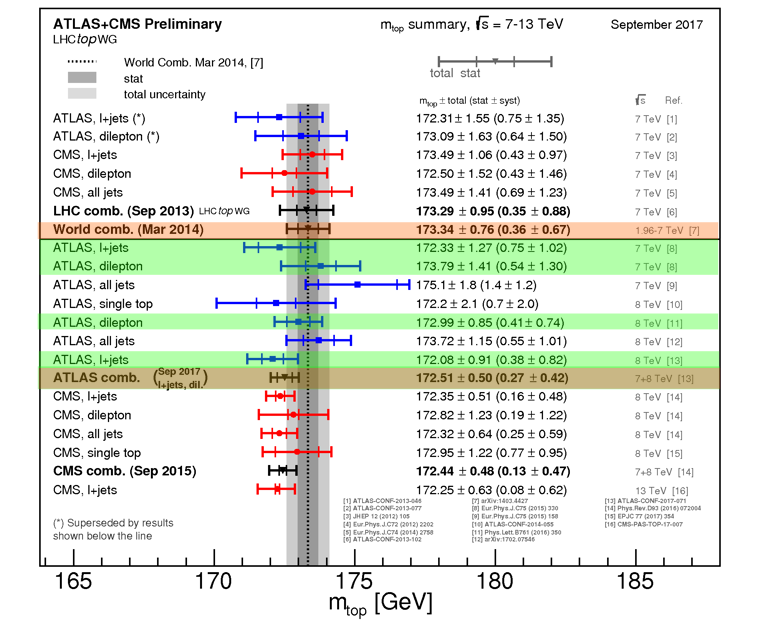
\includegraphics[width=0.9\linewidth]{Pics/mass}
	\caption{Summary of top-quark mass measurements, performed by the CMS and the ATLAS collaboration~\cite{PubR}. }
	
	\label{fig:mass}
\end{figure}



